\section{Model Representations}
\label{sec:representations}

The design of the \Treebeard{} compiler allows the implementation of different strategies for 
the in-memory representation of the model. The compiler currently has implementations for 
the three representations shown in Figure \ref{Fig:Representations}. The array and sparse 
representations are the ones described in the \TreebeardOLD{} paper\cite{Treebeard}. The reorg 
representation is the representation used by the RAPIDs library\cite{FIL}. 
The \textbf{array representation} is the simplest representation where the trees are stored in an array
in level order. The \textbf{sparse representation} stores the trees in a sparse format where 
memory is allocated only for nodes present in the tree and nodes contain pointers to their children. The \textbf{reorg representation}
interleaves the array representation of each tree in the model: all root nodes are stored first, then 
the left children of all the roots and so on. This representation was 
designed to improve memory coalescing when tree nodes are being loaded. 
\begin{figure}[htb]
  \centering
  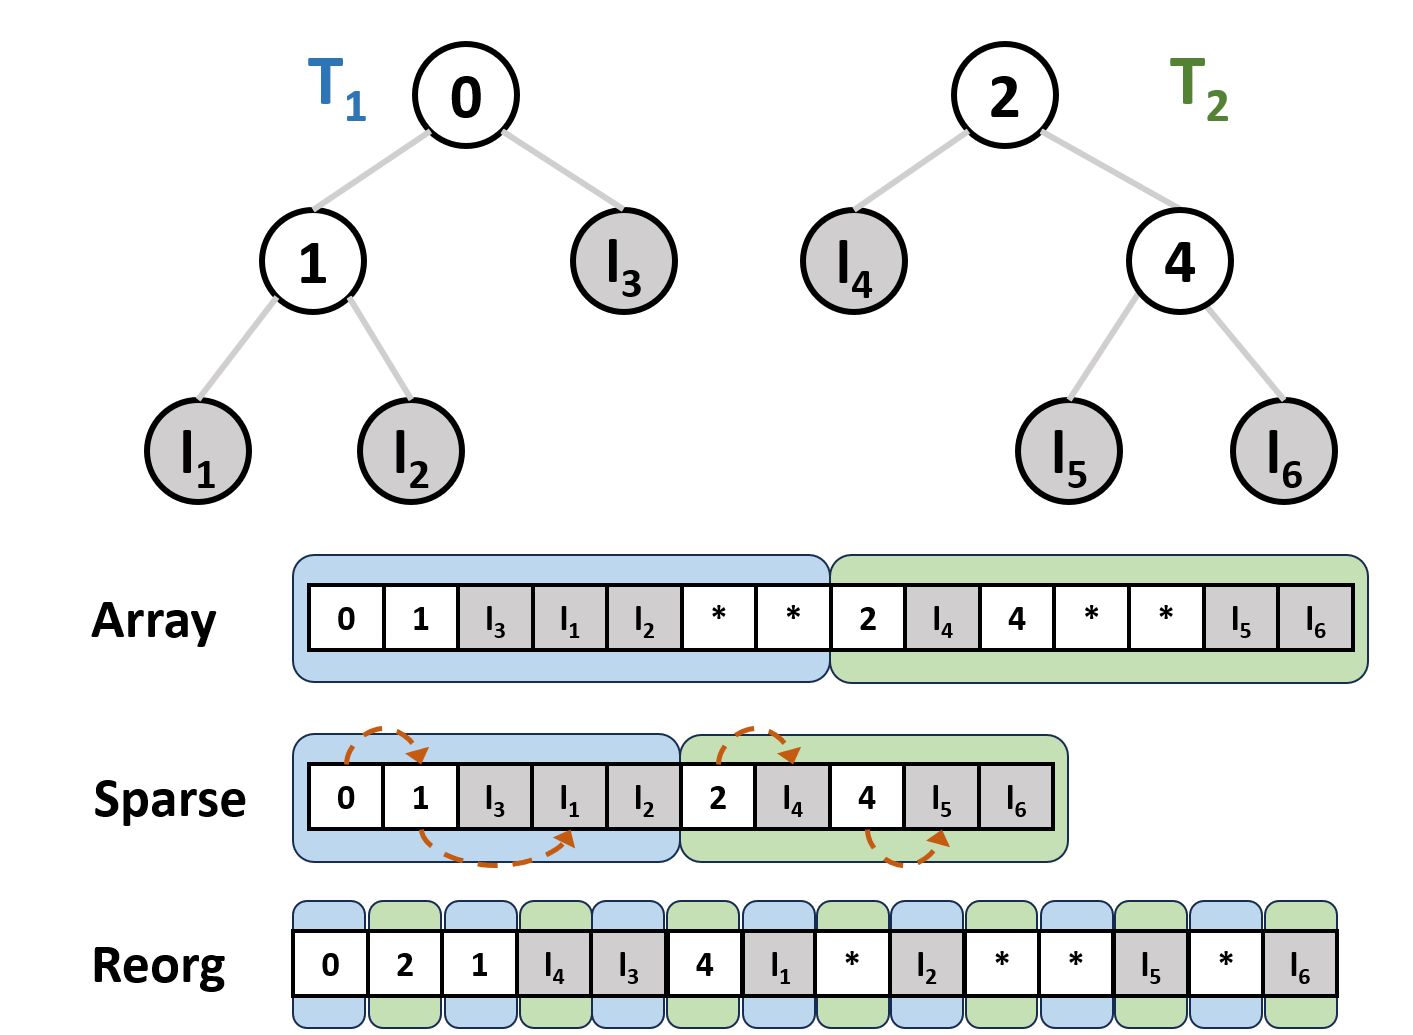
\includegraphics[width=\linewidth]{figures/representations.png}
  \caption{The three representations supported by \Treebeard{}.}
  \label{Fig:Representations}
\end{figure}

One of the major changes we make to the original design of \TreebeardOLD{} \cite{Treebeard} is to
separate the implementation of representations from the rest of the compiler. This allows
us to implement representations as plugins to the compiler. We define an interface 
that representations implement. The code generator is implemented using
this interface thus hiding details of the actual representation from the core 
compiler. Curcially, the interface abstracts how and what buffers 
are allocated, how to move from a node to its child, how trees 
are cached, reading the value of leaves and now threshold and 
feature indices are read from the allocated buffers.
% The interface abstracts the following details. 
% \begin{itemize}
%   \item \textbf{Buffer allocation:} The representation object exposes methods that generate 
%   buffer allocations in the IR. 
%   \item \textbf{Moving to child nodes:} Given the value of the predicate at a node (or tile),
%   generate code to move to the appropriate child node of the current node.
%   \item \textbf{Leaf representation:} The interface abstracts determining whether the current
%   node is a leaf (which is needed to terminate walks) and how to get the value of the leaf
%   (which is needed to get a tree's prediction).
%   \item \textbf{Caching trees:} Since reading the trees into shared memory on GPU (or prefetching)
%   them on CPU require knowledge of the buffer layout, the task of generating caching code for trees
%   is delegated to the representation object. 
%   \item \textbf{Loading thresholds and feature indices:} The representation object provides MLIR 
%   rewrite patterns to lower operations that load thresholds and feature indices to LLVM IR. This
%   is necessary because the details of how to load the thresholds and feature indices from the model 
%   buffers is representation-specific.
% \end{itemize}

In summary, the representation interface abstracts the details of how the model is stored in memory
and allows the compiler to generate code without having to explicitly know the details of the
representation. This design allows us to implement new representations without changing the core
compiler infrastructure. Implementing the representations as plugins also allows us to reuse
the implementations across different lowering pipelines. 

% For example, the code for the array 
% and sparse representations is almost fully shared between the CPU and GPU lowering pipelines.   

\section{Caching}
\label{sec:caching}

% \begin{itemize}
%   \item The compiler exposes caching of both trees and input rows in a unified manner.
%   \item This is independent of the final target on which the inference is to be run.
%   \item The caching is done at the granularity of a tree or a row.
%   \item Caching is encoded in the mid-level IR using the \op{cacheTrees} and \op{cacheRows} operations. 
%   These operations are generated when the HIR lowered to MIR and \op{Cache()} is specified on an 
%   index variable in the schedule. While the HIR is being lowered and a cached index variable is 
%   encountered, the compiler generates a \op{cacheTrees} or \op{cacheRows} operation depending on 
%   whether the index variable is a tree or a batch index variable.
%   \TODO{Should we talk about how the lowering from HIR to MIR is actually implemented as a tree walk?}
%   \item The lowering of these ops is done by the target-specific code generator.
%   \item For the \op{cacheRows} operation, \Treebeard{} uses pre-implemented lowerings for both
%   CPU and GPU. This is possible because the input is currently assumed to be a dense 
%   array format. 
%   \item For the \op{cacheTrees} operation, the lowering is representation-specific.
%   Each representation provides a lowering to the target-specific code generator
%   to lower the \op{cacheTrees} op when that representation is used.
%   \item The cache operations are lowered to reads into shared memory while compiling to GPU 
%   and to prefetches while compiling to CPU.
% \end{itemize}

\Treebeard{} provides mechanisms to cache both trees and input rows 
on both the CPU and GPU. As described in Section \ref{sec:schedule}, 
the user can specify that the working set of an iteration of a loop
needs to be cached using the \op{cache} directive. This 
provides a unified way to specify caching of both trees and input rows.
\Treebeard{} implements caching at the granularity of a tree or a row.

% \subsection{IR Representation of Caching}
Caching is encoded in the mid-level IR using the \op{cacheTrees} and \op{cacheRows} operations (Table \ref{Tab:IRSpecification}). 
These operations are generated when the HIR lowered to MIR and \op{cache} is specified on an 
index variable in the schedule. While the HIR is being lowered and a cached index variable is 
encountered, the compiler generates a \op{cacheTrees} or \op{cacheRows} operation depending on 
whether the index variable is a tree or a batch index variable.
\Treebeard{} also determines the working set of the loop  
and generates a caching operation with the appropriate limits.

% Each of the caching operations take parameters that specify the set of trees or rows that need 
% to be cached. The caching operations are defined as follows. 
% \begin{itemize}
%   \item \textbf{\op{cacheTrees(forest, start, end)}:} This operation caches the trees in ensemble
%   \op{forest} from \op{start} to \op{end}. The trees are cached in the order in which they are
%   specified in the ensemble. 
%   \item \textbf{\op{cacheRows(data, start, end)}:} This operation caches the rows in the input 
%   array \op{data} from \op{start} to \op{end}. The rows are cached in the same order as in the
%   input array.
% \end{itemize} 

%\subsection{Lowering of Caching Operations}
When the MIR is lowered to LIR, the cache ops are lowered to target-specific code. Each of 
the two caching operations is lowered differently for the CPU and the GPU. On CPU, the cahce operations are lowered to preteches while
on the GPU they are lowered to reads into shared memory.

Lowering the \op{cacheRows} operation is straightforward
% \Treebeard{} uses pre-implemented lowerings for both
% CPU and GPU. This is possible 
because the input is currently assumed to be a dense
array format. The lowering for the \op{cacheRows} operation is implemented directly in the \Treebeard{} compiler.

For the \op{cacheTrees} operation, the lowering is representation-specific. Each representation
provides a lowering to the target-specific code 
generator to lower the \op{cacheTrees} op when
that representation is used.
%  However, the \Treebeard{} infrastructure does provide helpers 
% to generate caching code to cache contiguous regions of memory. These helpers are reused 
% as required across different representations. 

\section{Exploring the Schedule Space}
\label{sec:exploring}

% \begin{itemize}
%   \item The scheduling language described in Section \ref{sec:schedule} allows
%   for numerous possible schedules for a given model. 
%   Finding a schedule with good performance is a non-trivial task.
%   \item We identify a reasonable template schedule for GPUs which encompasses
%   all strategies published in prior work.
%   \item Describe the template schedule.
%   \item Even within the variants of this template schedule, there is a significant 
%   amount of variation in performance. Show the histogram. 
%   \item Extensively exploring all possible parameter values for the template schedule 
%   is infeasible due to the large number of parameters.
%   Cite some numbers on how long it takes to explore the schedule space.
%   \item List the observations we make and the heuristic we design based on these.
% \end{itemize}

The set of schedules that can be constructed using the scheduling language described in 
Section \ref{sec:schedule} is vast. Searching this schedule space to find a schedule that
provides good performance is a non-trivial task. To simplify this process, we identify a
template schedule for GPUs that encompasses several strategies published in prior work.
Our template schedule assigns a fixed number of rows to each thread block and to each thread.
It distributes the trees across a fixed number of threads and can cache trees and 
input rows if required. Unrolling and interleaving of tree walks is also supported.

The template schedule exposes a number of parameters that can be tuned to find a 
high-performance schedule.
\begin{itemize}
  \item \textbf{Number of rows per thread block (Integer):} The number of rows that are processed by each thread block.
  \item \textbf{Number of rows per thread (Integer):} The number of rows processed by each thread.
  \item \textbf{Number of tree threads (Integer):} The number of threads across which the trees are distributed.
  \item \textbf{Cache rows (Boolean):} Whether the input rows are cached in shared memory.
  \item \textbf{Cache trees (Boolean):} Whether the trees are cached in shared memory.
  \item \textbf{Unroll walks (Boolean):} Whether the tree walks are unrolled.
  \item \textbf{Tree walk interleave factor:} The number of tree walks that are interleaved.
  \item \textbf{Shared memory reduction:} Whether the reduction across tree threads is done in shared memory.
\end{itemize}

While the template schedule simplifies optimization of generated inference code, it is 
important to note that the \Treebeard{} compiler itself does not place any 
restrictions on the schedule. The user is free to specify any schedule they wish.
The auto-scheduler that implements the template schedule is implemented as a 
module outside the core \Treebeard{} compiler. Users are also free to implement 
other auto-schedulers that generate schedules different from the template schedule.

\begin{figure}[htb]
  \centering
  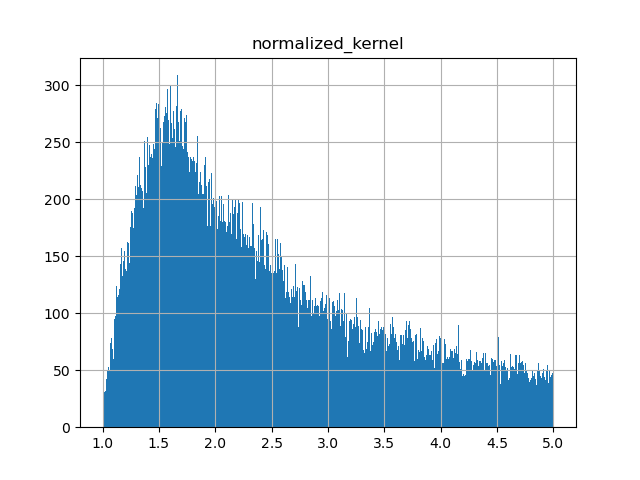
\includegraphics[width=\linewidth]{figures/normalized_kernel_histogram_lt5.png}
  \caption{Distribution of normalized execution times for all benchmark models
  with different parameter values for the template schedule. \TODO{We need to 
  describe exactly what the considered set of parameter values are.}}
  \label{Fig:ExecTimeDistribution}
\end{figure}

Figure \ref{Fig:ExecTimeDistribution} shows the distribution of normalized execution times
for all benchmark models with different parameter values for the template schedule.
The normalized execution time is the inference time of the model with a given set of
parameter values divided by the best inference time of the model.
The histogram shows that even within the variants of the template schedule, there is
a significant amount of variation in performance. Very few schedules perform close to the best
while a vast majority of schedules perform poorly.

Exploring the schedule space extensively even for a reasonable set of parameter values
is very expensive. We explored the set of parameter values listed in Table \ref{table:ParamVals}
for our benchmarks and found that it took anywhere between thirty minutes up to a few hours
to explore the entire space. Performing this extensive search for every model being compiled 
is infeasible in practise. We therefore need a better mechanism to guide the search for a good schedule.

We design a heuristic to narrow down the set of schedules to explore based on the following 
observations on high-performance schedules.
\begin{itemize}
  \item For small batch sizes, the best schedules tend to have a small number of rows
  per thread block and partition the trees across a larger number of threads. This is 
  intuitive since the amount of data parallelism across the rows is limited for small batch sizes.
  \item Always cache rows in shared memory and never cache trees. We find that caching rows 
  when possible (i.e., when the number of features is small enough to fit in shared memory)
  almost always improves performance. Caching trees on the other hand almost always degrades 
  performance. This is because the one time cost of loading trees into shared memory is 
  not sufficiently amortized when the whole of the tree is not accessed during inference. 
  \item Models with a large number of features tend to benefit from partitioning the 
  trees across more threads even at larger batch sizes. This is because processing fewer rows at a time 
  allows us to keep them in shared memory. We empirically find that the threshold for when 
  we should start partitioning the trees across more threads is when the number of features
  is greater than 100. 
  \item We find that when a model prefers schedules with shared reduction, the same schedules 
  without shared reduction are among the best performing schedules without shared reduction.
  We therefore are able to separate the evaluation of shared reduction by collecting the 
  best schedules without shared reduction and only evaluating shared reduction on them. 
  Evaluating the top 3 schedules for shared reduction is sufficient in practice.  
\end{itemize}

\Treebeard{} uses these observations to narrow down the set of schedules to explore. 
The pseudo-code for the current heuristic is shown in Algorithm \ref{alg:heuristic}.
The algorithm first computes a subset of thread block configurations in the function 
\op{TBConfigs}. A set of schedules based on these thread block configurations 
is then computed (\op{schedules}). The model is compiled with each of these schedules 
and then the resulting inference code is profiled. The three best performing schedules 
are collected and shared reduction is enabled on them and the resulting schedules evaluated.
The best schedule among all the evaluated schedules is selected as the schedule to use.
We find that this heuristic is able to find schedules that are close to the best schedules
but improves the search time by two orders of magnitude as we show in Section \ref{sec:HeuristicResults}.

\begin{algorithm}
  \caption{Heuristic to guide the search for a good schedule}
  \label{alg:heuristic}
  \begin{algorithmic}[1]
  \Procedure{TBConfigs}{$N_{batch}$, $N_f$}
    \State $T_{batch} \gets 2048, T_f \gets 128$
    \If {$N_{batch} \leq T_{batch}$}
      \State $rowsPerBlock \gets \{8, 32\}$
      \State $treeThreads \gets \{20, 50\}$
    \Else
      \If {$N_{f} \leq T_{f}$}
        \State $rowsPerBlock \gets \{32, 64\}$
        \State $treeThreads \gets \{2, 10\}$
      \Else
        \State $rowsPerBlock \gets \{8, 32\}$
        \State $treeThreads \gets \{20, 50\}$
      \EndIf
    \EndIf
    \State \Return $rowsPerBlock, treeThreads$
  \EndProcedure
  \\
  \State $bestSchedules \gets PriorityQueue(3)$
  \State $rowsPerTB, treeThreads \gets TBConfigs(N_{batch}, N_f)$
  \State $cacheRows \gets \text{True}$
  \State $cacheTrees \gets \text{False}$
  \State $interleaveFactors \gets \{1, 2, 4\}$
  \State $reps \gets \{array, sparse, reorg\}$
  \State $schedules \gets (rowsPerTB, treeThreads,$ \\
                          \hspace{1.5cm}$cacheRows, cacheTrees,$\\ 
                          \hspace{1.5cm}$interleaveFactors)$
  \For{$(sched, rep) \in schedules \times reps$}
    \State $time \gets EvaluateSchedule(sched, rep)$
    \State $bestSchedules.insert(time, sched, rep)$
  \EndFor
  \State $shMemSchedules \gets \emptyset$
  \For{$sched, rep \in bestSchedules$}
    \State $EnableSharedReduction(sched)$
    \State $time \gets EvaluateSchedule(sched, rep)$
    \State $shMemSchedules.insert(time, sched, rep)$
  \EndFor
  \State \Return $min(shMemSchedules \cup bestSchedules)$
  \end{algorithmic} 
\end{algorithm}